\subsection{Práctica N° 4}

\subsubsection{Puntos estaticos de operación amplificador multietapas}

\begin{table}[h!]
\centering
\begin{tabular}{|c|c|c|c|c|c|c|c|c|c|}
\hline
\textbf{Transistor} & \textbf{\(Vc[V]\)} & \textbf{\(\varDelta Vc[V]\)} & \textbf{\(Vb[V]\)} & \textbf{\(\varDelta Vb[V]\)} & \textbf{\(Ve[V]\)} & \textbf{\(\varDelta Ve[V]\)} & \textbf{\(Re[\Omega]\)} & \textbf{\(\varDelta Re[\Omega]\)} \\ \hline
Q1 & 7.2 & 0.4 & -0.016 & 0.002 & -0.6 & 0.04 & 4700 & 235 \\ \hline
Q2 & 7.6 & 0.4 & 0.048 & 0.004 & -0.64 & 0.04 & 4700 & 235 \\ \hline
Q3 & 7.6 & 0.4 & 8 & 1 & 9 & 1 & 6800 & 340 \\ \hline
Q4 & 0.68 & 0.04 & 0 & 0.1 & -0.56 & 0.04 & 5000 & 500 \\ \hline
Q5 & 10 & 1 & 0.6 & 0.1 & 0.1 & 0.02 & 20 & 1 \\ \hline
Q6 & -10 & 1 & -0.5 & 0.1 & 0.2 & 0.02 & 20 & 1 \\ \hline
\end{tabular}
\caption{Mediciones de voltaje amplificador multietapas en respuesta en frecuencia}
\label{tab:med-voltaje-amplificador-multietapas-respuesta-frecuencia}
\end{table}


\begin{table}[h!]
\centering
\begin{tabular}{|c|c|c|c|c|c|c|}
\hline
\textbf{Parámetro} & \textbf{Transistor} & \textbf{Valor Teórico} & \textbf{Medición} & \textbf{Incertidumbre} & \textbf{Error Absoluto} & \textbf{Error Relativo} \\ \hline
$I_{c}$ & Q1 & 0.00062 & 0.000595745 & 0.000231084 & 0.00002426 & 3.91\% \\ \hline
$I_{c}$ & Q2 & 0.00062 & 0.000510638 & 0.000230574 & 0.00010936 & 17.64\% \\ \hline
$I_{c}$ & Q3 & -0.00237 & -0.002588235 & 0.000204533 & 0.00021824 & 9.21\% \\ \hline
$I_{c}$ & Q4 & 3.02E-04 & 0.000112 & 2.42784E-05 & 0.00019036 & 62.96\% \\ \hline
$I_{c}$ & Q5 & 3.50E-04 & 0.005 & 0.001436141 & 0.00465000 & 1328.57\% \\ \hline
$I_{c}$ & Q6 & 3.50E-04 & 0.005 & 0.001436141 & 0.00465000 & 1328.57\% \\ \hline
$V_{ce}$ & Q1 & 7.79 & 7.8 & 0.401995025 & 0.01000000 & 0.13\% \\ \hline
$V_{ce}$ & Q2 & 7.79 & 8.24 & 0.401995025 & 0.45000000 & 5.78\% \\ \hline
$V_{ce}$ & Q3 & 2.27 & 1.4 & 1.077032961 & 0.87000000 & 38.33\% \\ \hline
$V_{ce}$ & Q4 & 1.24 & 1.24 & 0.056568542 & 0.00000000 & 0.00\% \\ \hline
$V_{ce}$ & Q5 & 9.99 & 9.9 & 1.00019998 & 0.09000000 & 0.90\% \\ \hline
$V_{ce}$ & Q6 & -9.99 & -10.2 & 1.00019998 & 0.21000000 & 2.10\% \\ \hline
\end{tabular}
\caption{Puntos estáticos de operación amplificador multietapa para respuesta en frecuencia}
\label{tab:med-puntos-estaticos-operacion-amplificador-multietapa-respuesta-frecuencia}
\end{table}


\subsubsection{Respuesta en frecuencia amplificador multietapas}

\begin{table}[h!]
\centering
\begin{tabular}{|c|c|c|c|c|c|c|}
\hline
\textbf{N} & \textbf{\(Vi[V]\)} & \textbf{\(\varDelta Vi[V]\)} & \textbf{\(Vo[V]\)} & \textbf{\(\varDelta Vo[V]\)} & \textbf{\(T\)} & \textbf{\(\varDelta T\)} \\ \hline
1 & 0.0032 & 0.0004 & 0.8 & 0.1 & 0.001 & 0.00004 \\ \hline
2 & 0.0032 & 0.0004 & 0.56 & 0.04 & 8.4E-05 & 0.002 \\ \hline
3 & 0.0032 & 0.0004 & 0.48 & 0.04 & 7.20046E-05 & 0.002 \\ \hline
4 & 0.0032 & 0.0004 & 0.56 & 0.04 & 0.014400922 & 0.0004 \\ \hline
5 & 0.0032 & 0.0004 & 0.36 & 0.04 & 0.0330033 & 0.001 \\ \hline
6 & 0.0032 & 0.0004 & 0.1 & 0.04 & 0.107991361 & 0.004 \\ \hline
7 & 0.0032 & 0.0004 & 0.6 & 0.04 & 0.011599582 & 0.0004 \\ \hline
8 & 0.0032 & 0.0004 & 0.76 & 0.04 & 0.005 & 0.0002 \\ \hline
9 & 0.0032 & 0.0004 & 0.68 & 0.04 & 0.00016 & 0.00001 \\ \hline
10 & 0.0032 & 0.0004 & 0.6 & 0.04 & 0.0001 & 0.000004 \\ \hline
11 & 0.0032 & 0.0004 & 0.48 & 0.04 & 7E-05 & 0.0000024 \\ \hline
\\ 
\\ \hline
\textbf{N} & \textbf{\(A\)} & \textbf{\(\varDelta A\)} & \textbf{\(A[dB]\)} & \textbf{\(\varDelta A[dB]\)} & \textbf{\(f[Hz]\)} & \textbf{\(\varDelta f[Hz]\)} \\ \hline
1 & 250 & 44.19417382 & 47.95880017 & 1.535462866 & 1000 & 40 \\ \hline
2 & 175 & 25.19455546 & 44.86076097 & 1.250497876 & 11904.76 & 283446.6213 \\ \hline
3 & 150 & 22.53469547 & 43.52182518 & 1.304892519 & 13888 & 385753.088 \\ \hline
4 & 175 & 25.19455546 & 44.86076097 & 1.250497876 & 69.44 & 1.92876544 \\ \hline
5 & 112.5 & 18.81499153 & 41.02305045 & 1.452666133 & 30.3 & 0.91809 \\ \hline
6 & 31.25 & 13.09613642 & 29.89700043 & 3.640051059 & 9.26 & 0.3429904 \\ \hline
7 & 187.5 & 26.5625 & 45.46002544 & 1.230501032 & 86.21 & 2.97286564 \\ \hline
8 & 237.5 & 32.2117627 & 47.51327228 & 1.178053962 & 200 & 8 \\ \hline
9 & 212.5 & 29.35670973 & 46.54717869 & 1.199948898 & 6250 & 390.625 \\ \hline
10 & 187.5 & 26.5625 & 45.46002544 & 1.230501032 & 10000 & 400 \\ \hline
11 & 150 & 22.53469547 & 43.52182518 & 1.304892519 & 14285.71 & 489.7956245 \\ \hline
\end{tabular}
\caption{Mediciones respuesta en frecuencia amplificador multietapas acoplado por condensadores}
\label{tab:med-respuesta-frecuencia-amplificador-multietapas-acoplado-condensadores}
\end{table}

\begin{table}[h!]
\centering
\begin{tabular}{|c|c|c|c|c|c|}
\hline
\textbf{Parámetro} & \textbf{Valor Teórico} & \textbf{Medición} & \textbf{Incertidumbre} & \textbf{Error Absoluto} & \textbf{Error Relativo} \\ \hline
$F_L$ [Hz] & 70.41 & 69.44 & 1.92876544 & 0.97000000 & 1.38\% \\ \hline
$H_H$ [Hz] & 10890 & 11904.76 & 283446.6213 & 1014.76000000 & 9.32\% \\ \hline
\end{tabular}
\caption{Medición de frecuencias de corte}
\label{tab:med-frecuencias-corte}
\end{table}


\begin{figure}[ht]
    \centering
    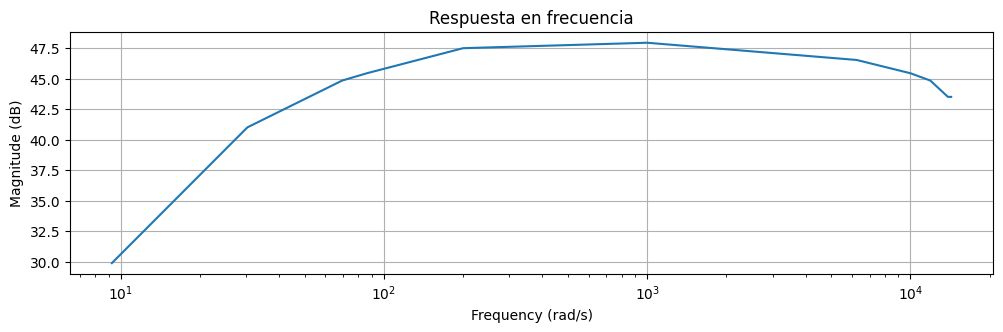
\includegraphics[width=0.8\textwidth]{src/images/resultados/p4/respuesta en frecuencia practica 4 con condensadores.png}
    \caption{Respuesta en frecuencia amplificador multietapas acoplado por condensadores}
    \label{fig:respuesta-frecuencia-amplificador-multietapas-acoplado-condensadores}
\end{figure}

\begin{figure}[ht]
    \centering
    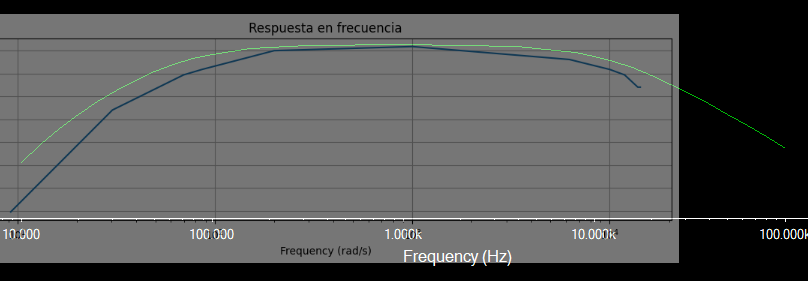
\includegraphics[width=0.8\textwidth]{src/images/resultados/p4/superposicion respuesta en frecuencia con condensadores.png}
    \caption{Superposición de respuesta en frecuencia amplificador multietapas acoplado por condensadores con su simulación}
    \label{fig:superposicion-respuesta-frecuencia-amplificador-multietapas-acoplado-condensadores}
\end{figure}

\subsubsection{Respuesta en frecuencia amplificador multietapas sin condensadores de acople}

\begin{table}[h!]
\centering
\begin{tabular}{|c|c|c|c|c|c|c|}
\hline
\textbf{N} & \textbf{\(Vi[V]\)} & \textbf{\(\varDelta Vi[V]\)} & \textbf{\(Vo[V]\)} & \textbf{\(\varDelta Vo[V]\)} & \textbf{\(T\)} & \textbf{\(\varDelta T\)} \\ \hline
1 & 1 & 0.1 & 0.026 & 0.002 & 0.001 & 0.00004 \\ \hline
2 & 1 & 0.1 & 0.0072 & 0.0004 & 0.006024096 & 0.0002 \\ \hline
3 & 1 & 0.1 & 0.01 & 0.001 & 0.003003003 & 0.0001 \\ \hline
4 & 1 & 0.1 & 0.015 & 0.001 & 0.002304147 & 0.0001 \\ \hline
5 & 1 & 0.1 & 0.024 & 0.002 & 0.001499993 & 0.0001 \\ \hline
6 & 1 & 0.1 & 0.034 & 0.002 & 0.00076 & 0.00004 \\ \hline
7 & 1 & 0.1 & 0.052 & 0.004 & 0.0005 & 0.00002 \\ \hline
8 & 1 & 0.1 & 0.09 & 0.01 & 0.00025 & 0.00001 \\ \hline
9 & 1 & 0.1 & 0.14 & 0.01 & 0.0001 & 0.000004 \\ \hline
10 & 1 & 0.1 & 0.15 & 0.01 & 5.99988E-05 & 0.000004 \\ \hline
11 & 1 & 0.1 & 0.15 & 0.01 & 0.00005 & 0.000002 \\ \hline
12 & 1 & 0.1 & 0.15 & 0.01 & 0.0001 & 0.00000014 \\ \hline
&&&&&&\\ \hline
\textbf{N} & \textbf{\(A\)} & \textbf{\(\varDelta A\)} & \textbf{\(A[dB]\)} & \textbf{\(\varDelta A[dB]\)} & \textbf{\(f[Hz]\)} & \textbf{\(\varDelta f[Hz]\)} \\ \hline
1 & 0.026 & 0.003280244 & -31.70053304 & 1.095839863 & 1000 & 40 \\ \hline
2 & 0.0072 & 0.00082365 & -42.85335007 & 0.99363008 & 166 & 5.5112 \\ \hline
3 & 0.01 & 0.001414214 & -40 & 1.228370293 & 333 & 11.0889 \\ \hline
4 & 0.015 & 0.001802776 & -36.47817482 & 1.043914015 & 434 & 18.8356 \\ \hline
5 & 0.024 & 0.0031241 & -32.39577517 & 1.130649446 & 666.67 & 44.44488889 \\ \hline
6 & 0.034 & 0.003944617 & -29.37042166 & 1.007720715 & 1315.79 & 69.25213296 \\ \hline
7 & 0.052 & 0.006560488 & -25.67993313 & 1.095839863 & 2000 & 80 \\ \hline
8 & 0.09 & 0.013453624 & -20.91514981 & 1.298407708 & 4000 & 160 \\ \hline
9 & 0.14 & 0.017204651 & -17.07743929 & 1.067412113 & 10000 & 400 \\ \hline
10 & 0.15 & 0.018027756 & -16.47817482 & 1.043914015 & 16667 & 1111.155556 \\ \hline
11 & 0.15 & 0.018027756 & -16.47817482 & 1.043914015 & 20000 & 800 \\ \hline
12 & 0.15 & 0.018027756 & -16.47817482 & 1.043914015 & 10000 & 14 \\ \hline
\end{tabular}
\caption{Mediciones respuesta en frecuencia amplificador multietapas sin condensadores de acople}
\label{tab:med-respuesta-frecuencia-amplificador-multietapas-sin-condensadores-acople}
\end{table}

\begin{figure}[ht]
    \centering
    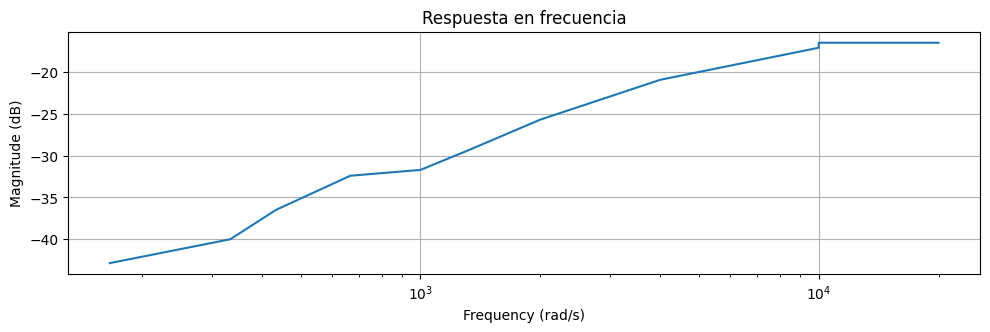
\includegraphics[width=0.8\textwidth]{src/images/resultados/p4/respuesta en frecuencia practica 4 sin condensadores de acople.png}
    \caption{Respuesta en frecuencia amplificador multietapas acoplado sin condensadores}
    \label{fig:respuesta-frecuencia-amplificador-multietapas-acoplado-sin-condensadores}
\end{figure}
